\documentclass{article}
\usepackage[utf8]{inputenc}

\usepackage{geometry}
\usepackage{float}
\usepackage{siunitx}

\usepackage{multirow}
\usepackage{subfig}
\usepackage{rotating}

\newgeometry{margin=2.5cm}
\newcommand\todo[1]{\textbf{TODO: #1}}


\title{Representative Wind Profiles Initial Findings}
\author{Mark Muetzelfeldt}
\date{February 2018}

\begin{document}

\maketitle

\section{Introduction}



\subsection{Motivation}

% GOAL: link grid-column WP to degree of subgrid shear-induced cloud field org.

% why wind profiles
% why shear important for mesoscale org
% what WPs get created by climate models
% explain WP space is large
% explain choice of clustering as data-driven, non-arbitrary was of grouping together WPs into RWPs to reduce space

\begin{itemize}
    \item subgrid org rarely represented in convection parametrization schemes climate models.
    \item one form of org is through shear-induced organization
    \item shear-induced org can cause the formation of MCSs such as squall lines, MCCs and MCVs \cite{houze2004mesoscale}
    \item MCSs important because of: large-scale, time correlation, high rainfall \todo{work on this}
    \item to represent this in a convection parametrization scheme, you need to be able to relate the grid-column wind profile to its subgrid organizational state
    \item however, there are a large number of possible WPs (WP space is large)
    \item by using clustering into RWPs, we reduce this space to a manageable number
    \item this clustering is driven by the grid-column state; it is not some arbitrary function of location (mid-latitude, over land etc).
    \item each RWP can then be used to drive a high-resolution RCE experiment
    \item important aspects of the cloud field organization - the cloud lifetime, the bulk entrainment rate - can then be measured from high-resolution experiments
    \item in the convection parametrization scheme, we can classify each grid-column WP
    \item based on the information from the high-resolution experiments, we can modify the convection parametrization scheme
\end{itemize}

\section{Methods}

\subsection{Model}

\begin{itemize}
    \item MO UM vn10.9
    \item GA7.0
    \item N96 + horizontal resolution at equator (around \SI{209}{km})
    \item N96 has a total of $145 \times 192$ grid points
    \item Run for \SI{1}{month}
    \item Run on ARCHER using u-au197 (copy of u-ar683, standard GA7.0 suite), archived to RDF (\todo{paths})
    \item $u$, $v$ and $w$ output on 7 pressure levels: \SIlist{950;900;850;800;700;600;500}{hPa}
    \item CAPE also output
    \item diagnostics output every \SI{6}{hr}, which gives a total of (4 * 30 * 145 * 192) \si{3340800} profiles
\end{itemize}

\subsection{Clustering procedure}

\todo{Broad overview of clustering, what it is, what it is not. Say I am using non-hierarchical clustering, justify this.}

\subsubsection{Filtering}

Profiles are filtered based on several criteria. The filters reduce the number of profiles, excluding ones that are not of interest for one reason or another. The filters in use are as follows:

\begin{enumerate}
    \item include grid points in the Tropics, defined as \ang{30}N and \ang{30}S;
    \item exclude grid points where CAPE \textless \SI{500}{J.kg^{-1}}; \todo{[PC] This is quite high; try reducing}
    \item exclude grid points where the maximum shear in the profile is less than the 25\textsuperscript{th} percentile.
\end{enumerate} 


\subsubsection{Normalization}
\label{sec:normalization}

It is desirable to normalize the data before performing the principal component analysis and the clustering. Two types of normalization are applied:

\paragraph{Magnitude:}

this is to ensure that differences in the profiles at each pressure level each contribute the same amount to the distance measure used by the KMA \todo{mention in Clustering procedure}. This involves normalizing each profile by the maximum magnitude of the wind at each pressure level (i.e. $\sqrt{u^2 + v^2}$).

It is true that the shape of the profiles is changed by the normalization; some concerns were raised by RP and PC that this could change the shear values for the profiles. It does change this shape, but it keeps the relative differences between the different profiles. Therefore, when the KMA is applied, it will still cluster like profiles together, based on its distance metric.

\paragraph{Rotation:}

this is applied to treat profiles that share rotational symmetry in the same way. It is done by using the wind vector at \SI{850}{hPa} to define a rotation angle. All profiles are then rotated so that this angle is zero, i.e. all the profiles are aligned in the same direction at \SI{850}{hPa}. A small number of profiles (4\% \todo{more precise}) have a wind magnitude less than \SI{1}{m.s^{-1}} at \SI{850}{hPa}, these profiles are included but it should be noted that they may influence results. After applying this normalization, $u$ refers to the direction aligned with the wind vector at \SI{850}{hPa}, and $v$ is the orthogonal direction to this.

The reason for applying this normalization is that in the Tropics, it makes little difference whether a profile has e.g. unidirectional shear in the zonal or meridional direction. A similar point stands for all profiles, such as profiles that veer/back with height. This will apply exactly only at the Equator; as the Coriolis parameter increases in magnitude, there will be some differences between rotated profiles. For the sake of this analysis, we are ignoring these. Also, in the high-resolution experiments that follow, we will be running experiments where $f = 0$.

\subsubsection{Principal component analysis}

PCA is a process that finds orthogonal, unit length principal components of a dataset that are linear combinations of the original axes. It does this in such a way that the first principal component accounts for the largest possible variance in the underlying dataset. The second principal component is orthogonal to the first, and accounts for the as much of the remaining variance as possible in the dataset, and so on. PCA can be used to reduce the number of dimensions of a dataset in a way the keeps the maximum possible variance for a given number of dimensions, by truncating the number of principal components used. In Meteorology, PCA is also known as Empirical Orthogonal Functions (EOF), when it is applied to geographical datasets to look for the dominant modes of variability, e.g. the North Atlantic Oscillation.

The algorithm for PCA works by centring the dataset on the mean for each of its dimensions, and then calculating the covariance matrix for this dataset. The principal components can then be taken by finding the eigenvectors of the covariance matrix, with the first component corresponding to the eigenvector with the highest eigenvalue, and so on. 

The number of dimensions of the original dataset is 14 (7 pressure levels for $u$ and $v$). We have chosen to keep as many principal components that are required to explain 90\% of the variance, for this dataset this is 4. These 4 principal components are shown in Fig. \ref{fig:pca_components}. \todo{say something about these PCs}.

\begin{figure}[htp!]%
    \centering
    \subfloat[PC 1]{{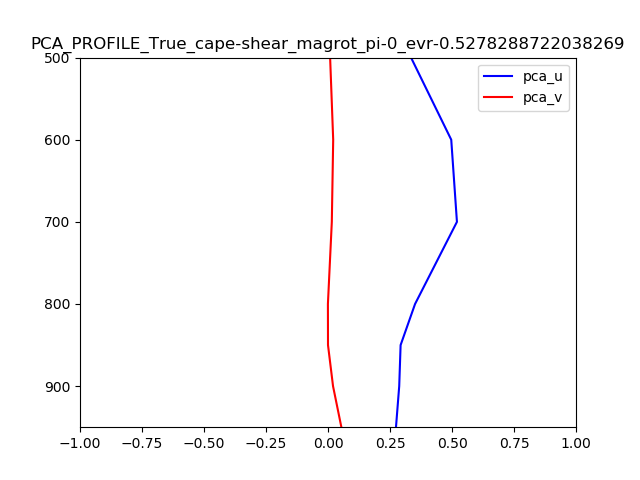
\includegraphics[width=7cm]{figs/PCA_PROFILE_True_cape-shear_magrot_pi-0} }}%
    \qquad
    \subfloat[PC 2]{{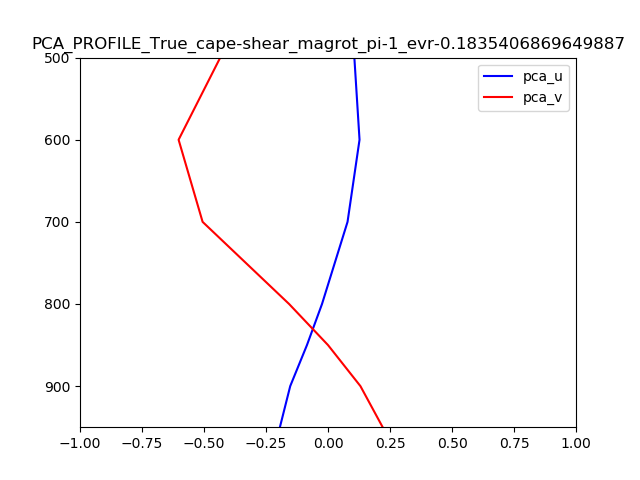
\includegraphics[width=7cm]{figs/PCA_PROFILE_True_cape-shear_magrot_pi-1} }}%
    \qquad
    \subfloat[PC 3]{{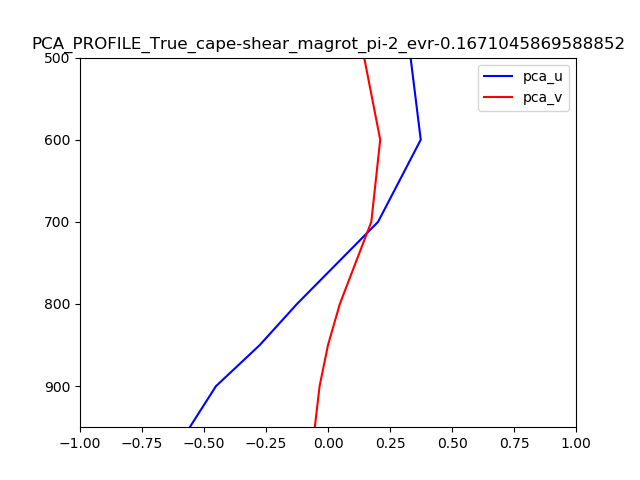
\includegraphics[width=7cm]{figs/PCA_PROFILE_True_cape-shear_magrot_pi-2} }}%
    \qquad
    \subfloat[PC 4]{{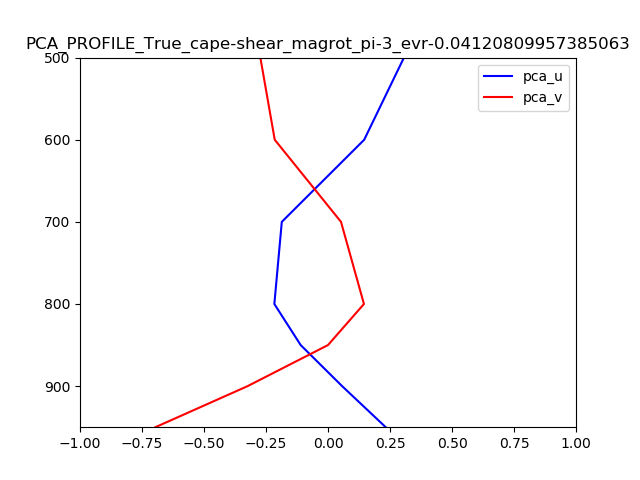
\includegraphics[width=7cm]{figs/PCA_PROFILE_True_cape-shear_magrot_pi-3} }}%
    \qquad
    \caption{The first 4 principal components.}%
    \label{fig:pca_components}%
\end{figure}

It is also insightful to look at the profiles that are produced by reprojecting the original profile along only these first 4 principal components. Some examples showing high and low fidelity to the original profiles are shown in Fig. \ref{fig:pca_reprojections}. \todo{some basic stats of how good keeping the first 4 components is? Or is this implicit in the fact that I have chosen to keep 90\% of the variance.}

\begin{figure}[htp!]%
    \centering
    \subfloat[]{{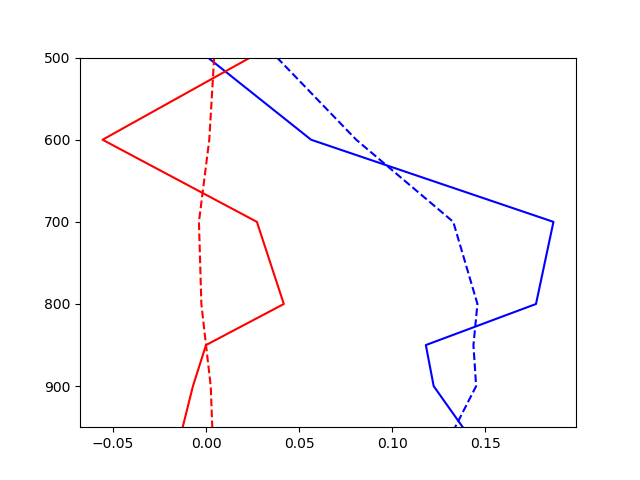
\includegraphics[width=7cm]{figs/PCA_RED_True_cape-shear_magrot_725164_-4_nclust-11_prof-3452.png} }}%
    \qquad
    \subfloat[]{{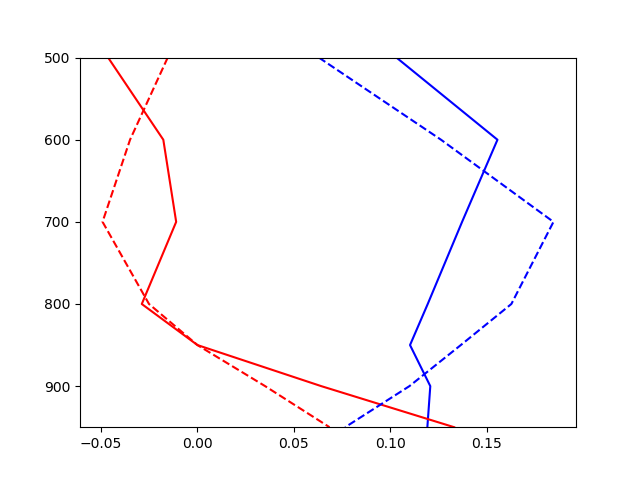
\includegraphics[width=7cm]{figs/PCA_RED_True_cape-shear_magrot_725164_-4_nclust-11_prof-7767} }}%
    \qquad
    \subfloat[]{{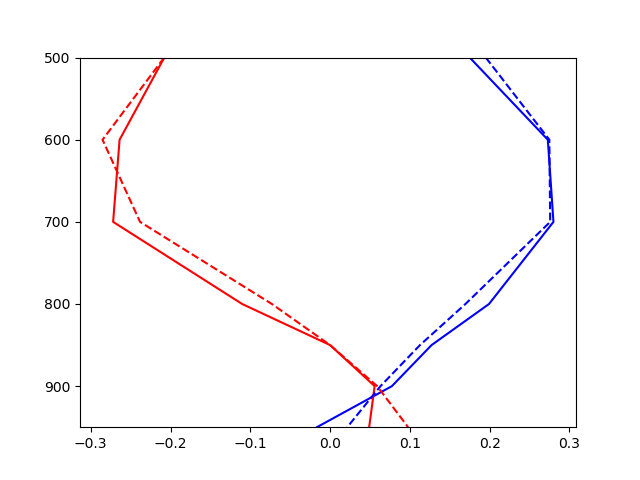
\includegraphics[width=7cm]{figs/PCA_RED_True_cape-shear_magrot_725164_-4_nclust-11_prof-5178} }}%
    \qquad
    \subfloat[]{{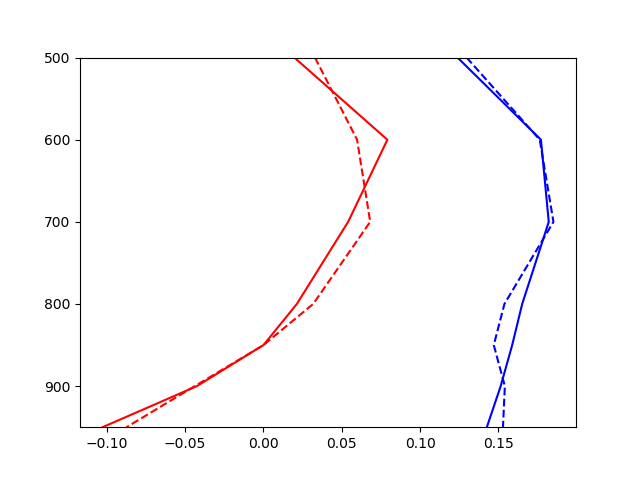
\includegraphics[width=7cm]{figs/PCA_RED_True_cape-shear_magrot_725164_-4_nclust-11_prof-12082} }}%
    \qquad
    \caption{4 profiles that have been re-projected using the first 4 principal components.}%
    \label{fig:pca_components}%
\end{figure}

\subsubsection{K-means clustering}

The K-means clustering algorithm (KMA) splits a number of samples \todo{haven't defined} into clusters based on how similar the samples are to other samples. It does this in a way which minimizes the within cluster variance. The algorithm used here is LLoyd's algorithm, which is computationally efficient but not guaranteed to find a global minimum for the within cluster variance. It starts by randomly assigning samples to clusters. Then it calculates the mean of each cluster, and then it re-assigns samples to new clusters based in which of the cluster means each sample is nearest to \todo{define distance metric somewhere}. This last step is repeated until there is very little movement (less than some predefined threshold) in the cluster means, when the algorithm terminates.

The number of clusters to use is not \textit{a priori} obvious. We have the competing requirements that we want few enough RWPs that we can analyse where each one comes from without being overloaded with data, and we want each RWP to be as representative as possible of its cluster of profiles. One method for working out a suitable number of clusters is known as the elbow method. This involves plotting the sum of the variances of each cluster, the score, against the number of clusters used. This will necessarily decrease in magnitude as the number of clusters increases, however, if there is a change in the rate of change in the gradient (a so-called `elbow'), then this indicates that using more clusters is reducing the score by a lower amount, and thus indicates a suitable number of clusters. Figure \ref{fig:kmeans_scores} shows the scores for 5-20 clusters. Although there is not a large elbow in this figure, there is a recognizable kink at 8 clusters and 11 clusters. We pick 11 clusters as a pragmatic number of clusters to use, being large enough to span the wind profile space, and small enough that sensible analysis of each cluster is possible.

\begin{figure}[h]
    \centering
    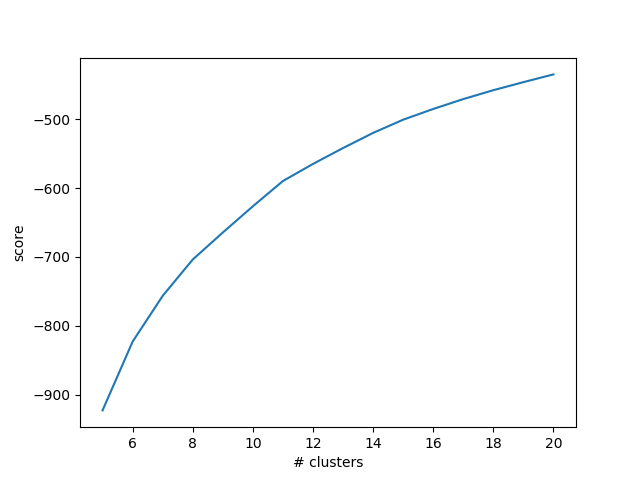
\includegraphics[width=400px]{figs/KMEANS_SCORES_True_cape-shear_magrot.png}
    \caption{}
    \label{fig:kmeans_scores}
\end{figure}

\section{Results}

\subsection{Representative Wind Profiles}

\section{Discussion}

\newpage
\section*{Appendix}

\subsection*{Background}

This is a short document that gives some history and technical details of the clustering work that I did from September 2017 to February 2018. The idea was that I needed to be able to link the grid-column state of a parametrized model to the subgrid shear-induced organizational state. The broad method I was trying was to investigate the wind profiles (WPs) produced by the model, and cluster these into Representative Wind Profiles (RWPs). This would reduce the `wind profile space' from a space that was too large to analyse to say 20 RWPs. Each of these RWPs could then be used to drive an RCE experiment, and then I could use the information from these experiments (such as cloud lifetimes) to feedback into the convection parametrization scheme. (This is future work.)

Initial results from last year were promising, using an sklearn K-means clustering algorithm (KMA), working on the standard output $u$ and $v$ fields at 6 pressure levels (\todo{what were they?}) collected every \SI{6}{hr} over the course of \SI{1}{month} of simulation. I only considered profiles between \ang{30}N and \ang{30}S over all longitudes. I filtered out profiles having a CAPE of less than \SI{500}{J.kg^{-1}}, or profiles with $w$ \textgreater  \SI{0}{m.s^{-1}}. I found the principal components of the profiles (using PCA), and used this to reduce the number of dimensions from 12 to around 4 (which explained over 90 \% of the variance). This was done as an advised precursor to using the KMA, as an attempt to reduce the impact of the so-called `curse of dimensionality', and additionally there is interesting information in the shape of the principal components. I made it so that I could quickly experiment with e.g. running with or without filtering, PCA etc. Choosing 20 clusters for the KMA, and plotting all the WPs for each RWP, it was believable that each cluster did capture some information about the underlying WP sample space, and that the RWPs could be of interest. Initially I was plotting every profile ($u$ and $v$) for each cluster, which made it hard to get a sense of what the mean profile looked like, although did not hide any information away. I have switched to plotting the mean, the mean +/- 1 standard deviation, and the 25\% and 75\% lines. N.B. it is easy to produce figures/results for each combination of options you can think of; it is harder to analyse them all. 

However, the profiles went too high into the atmosphere (\todo{what pressure?}), and because of this the clustering was being dominated by the high-level winds. To improve this, the profiles now only go up to \SI{500}{hPa}. Also, we worked out that we probably did not care about the relative orientation of the different WPs, and additionally we perhaps did not care about the sense of rotation (clockwise or anti-clockwise). I have now normalized for the orientation of the profiles, but not for the sense of rotation. I can also now filter on multiple attributes, and am now filtering on both CAPE and the maximum wind shear of each profile has to be greater than the lowest 25 \% of profiles. Additionally, I am normalizing the profiles on their magnitude at each pressure level separately (see Section \ref{sec:normalization} for more details and justification).


\end{document}
